\documentclass[1p]{elsarticle_modified}
%\bibliographystyle{elsarticle-num}

%\usepackage[colorlinks]{hyperref}
%\usepackage{abbrmath_seonhwa} %\Abb, \Ascr, \Acal ,\Abf, \Afrak
\usepackage{amsfonts}
\usepackage{amssymb}
\usepackage{amsmath}
\usepackage{amsthm}
\usepackage{scalefnt}
\usepackage{amsbsy}
\usepackage{kotex}
\usepackage{caption}
\usepackage{subfig}
\usepackage{color}
\usepackage{graphicx}
\usepackage{xcolor} %% white, black, red, green, blue, cyan, magenta, yellow
\usepackage{float}
\usepackage{setspace}
\usepackage{hyperref}

\usepackage{tikz}
\usetikzlibrary{arrows}

\usepackage{multirow}
\usepackage{array} % fixed length table
\usepackage{hhline}

%%%%%%%%%%%%%%%%%%%%%
\makeatletter
\renewcommand*\env@matrix[1][\arraystretch]{%
	\edef\arraystretch{#1}%
	\hskip -\arraycolsep
	\let\@ifnextchar\new@ifnextchar
	\array{*\c@MaxMatrixCols c}}
\makeatother %https://tex.stackexchange.com/questions/14071/how-can-i-increase-the-line-spacing-in-a-matrix
%%%%%%%%%%%%%%%

\usepackage[normalem]{ulem}

\newcommand{\msout}[1]{\ifmmode\text{\sout{\ensuremath{#1}}}\else\sout{#1}\fi}
%SOURCE: \msout is \stkout macro in https://tex.stackexchange.com/questions/20609/strikeout-in-math-mode

\newcommand{\cancel}[1]{
	\ifmmode
	{\color{red}\msout{#1}}
	\else
	{\color{red}\sout{#1}}
	\fi
}

\newcommand{\add}[1]{
	{\color{blue}\uwave{#1}}
}

\newcommand{\replace}[2]{
	\ifmmode
	{\color{red}\msout{#1}}{\color{blue}\uwave{#2}}
	\else
	{\color{red}\sout{#1}}{\color{blue}\uwave{#2}}
	\fi
}

\newcommand{\Sol}{\mathcal{S}} %segment
\newcommand{\D}{D} %diagram
\newcommand{\A}{\mathcal{A}} %arc


%%%%%%%%%%%%%%%%%%%%%%%%%%%%%5 test

\def\sl{\operatorname{\textup{SL}}(2,\Cbb)}
\def\psl{\operatorname{\textup{PSL}}(2,\Cbb)}
\def\quan{\mkern 1mu \triangleright \mkern 1mu}

\theoremstyle{definition}
\newtheorem{thm}{Theorem}[section]
\newtheorem{prop}[thm]{Proposition}
\newtheorem{lem}[thm]{Lemma}
\newtheorem{ques}[thm]{Question}
\newtheorem{cor}[thm]{Corollary}
\newtheorem{defn}[thm]{Definition}
\newtheorem{exam}[thm]{Example}
\newtheorem{rmk}[thm]{Remark}
\newtheorem{alg}[thm]{Algorithm}

\newcommand{\I}{\sqrt{-1}}
\begin{document}

%\begin{frontmatter}
%
%\title{Boundary parabolic representations of knots up to 8 crossings}
%
%%% Group authors per affiliation:
%\author{Yunhi Cho} 
%\address{Department of Mathematics, University of Seoul, Seoul, Korea}
%\ead{yhcho@uos.ac.kr}
%
%
%\author{Seonhwa Kim} %\fnref{s_kim}}
%\address{Center for Geometry and Physics, Institute for Basic Science, Pohang, 37673, Korea}
%\ead{ryeona17@ibs.re.kr}
%
%\author{Hyuk Kim}
%\address{Department of Mathematical Sciences, Seoul National University, Seoul 08826, Korea}
%\ead{hyukkim@snu.ac.kr}
%
%\author{Seokbeom Yoon}
%\address{Department of Mathematical Sciences, Seoul National University, Seoul, 08826,  Korea}
%\ead{sbyoon15@snu.ac.kr}
%
%\begin{abstract}
%We find all boundary parabolic representation of knots up to 8 crossings.
%
%\end{abstract}
%\begin{keyword}
%    \MSC[2010] 57M25 
%\end{keyword}
%
%\end{frontmatter}

%\linenumbers
%\tableofcontents
%
\newcommand\colored[1]{\textcolor{white}{\rule[-0.35ex]{0.8em}{1.4ex}}\kern-0.8em\color{red} #1}%
%\newcommand\colored[1]{\textcolor{white}{ #1}\kern-2.17ex	\textcolor{white}{ #1}\kern-1.81ex	\textcolor{white}{ #1}\kern-2.15ex\color{red}#1	}

{\Large $\underline{12a_{0584}~(K12a_{0584})}$}

\setlength{\tabcolsep}{10pt}
\renewcommand{\arraystretch}{1.6}
\vspace{1cm}\begin{tabular}{m{100pt}>{\centering\arraybackslash}m{274pt}}
\multirow{5}{120pt}{
	\centering
	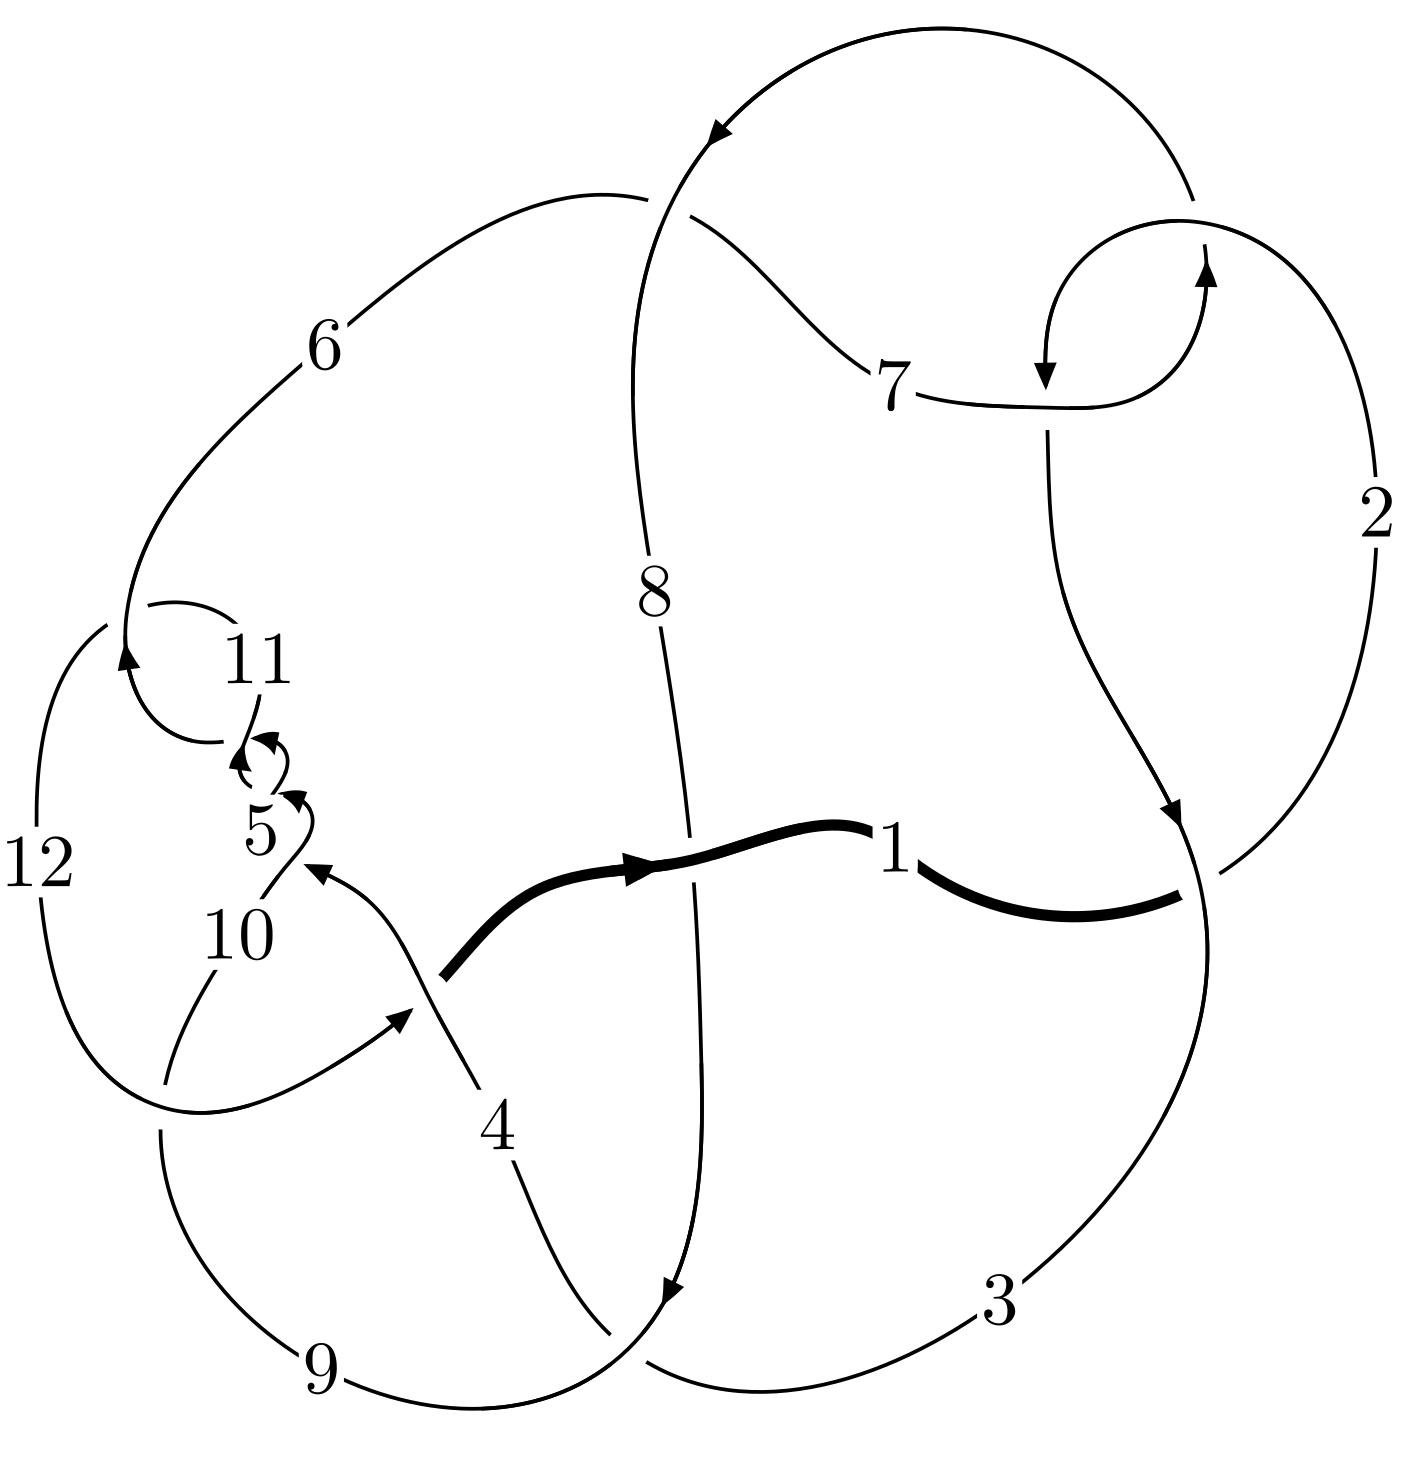
\includegraphics[width=112pt]{../../../GIT/diagram.site/Diagrams/png/1385_12a_0584.png}\\
\ \ \ A knot diagram\footnotemark}&
\allowdisplaybreaks
\textbf{Linearized knot diagam} \\
\cline{2-2}
 &
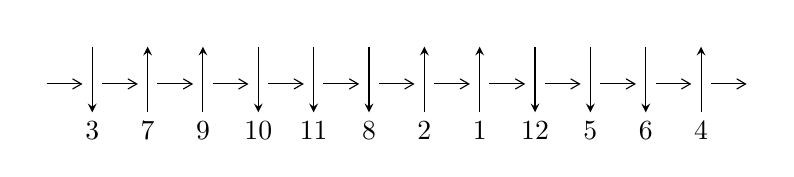
\begin{tikzpicture}[x=20pt, y=17pt]
	% nodes
	\node (C0) at (0, 0) {};
	\node (C1) at (1, 0) {};
	\node (C1U) at (1, +1) {};
	\node (C1D) at (1, -1) {3};

	\node (C2) at (2, 0) {};
	\node (C2U) at (2, +1) {};
	\node (C2D) at (2, -1) {7};

	\node (C3) at (3, 0) {};
	\node (C3U) at (3, +1) {};
	\node (C3D) at (3, -1) {9};

	\node (C4) at (4, 0) {};
	\node (C4U) at (4, +1) {};
	\node (C4D) at (4, -1) {10};

	\node (C5) at (5, 0) {};
	\node (C5U) at (5, +1) {};
	\node (C5D) at (5, -1) {11};

	\node (C6) at (6, 0) {};
	\node (C6U) at (6, +1) {};
	\node (C6D) at (6, -1) {8};

	\node (C7) at (7, 0) {};
	\node (C7U) at (7, +1) {};
	\node (C7D) at (7, -1) {2};

	\node (C8) at (8, 0) {};
	\node (C8U) at (8, +1) {};
	\node (C8D) at (8, -1) {1};

	\node (C9) at (9, 0) {};
	\node (C9U) at (9, +1) {};
	\node (C9D) at (9, -1) {12};

	\node (C10) at (10, 0) {};
	\node (C10U) at (10, +1) {};
	\node (C10D) at (10, -1) {5};

	\node (C11) at (11, 0) {};
	\node (C11U) at (11, +1) {};
	\node (C11D) at (11, -1) {6};

	\node (C12) at (12, 0) {};
	\node (C12U) at (12, +1) {};
	\node (C12D) at (12, -1) {4};
	\node (C13) at (13, 0) {};

	% arrows
	\draw[->,>={angle 60}]
	(C0) edge (C1) (C1) edge (C2) (C2) edge (C3) (C3) edge (C4) (C4) edge (C5) (C5) edge (C6) (C6) edge (C7) (C7) edge (C8) (C8) edge (C9) (C9) edge (C10) (C10) edge (C11) (C11) edge (C12) (C12) edge (C13) ;	\draw[->,>=stealth]
	(C1U) edge (C1D) (C2D) edge (C2U) (C3D) edge (C3U) (C4U) edge (C4D) (C5U) edge (C5D) (C6U) edge (C6D) (C7D) edge (C7U) (C8D) edge (C8U) (C9U) edge (C9D) (C10U) edge (C10D) (C11U) edge (C11D) (C12D) edge (C12U) ;
	\end{tikzpicture} \\
\hhline{~~} \\& 
\textbf{Solving Sequence} \\ \cline{2-2} 
 &
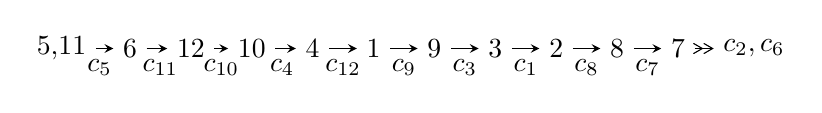
\begin{tikzpicture}[x=22pt, y=7pt]
	% node
	\node (A0) at (-1/8, 0) {5,11};
	\node (A1) at (1, 0) {6};
	\node (A2) at (2, 0) {12};
	\node (A3) at (3, 0) {10};
	\node (A4) at (4, 0) {4};
	\node (A5) at (5, 0) {1};
	\node (A6) at (6, 0) {9};
	\node (A7) at (7, 0) {3};
	\node (A8) at (8, 0) {2};
	\node (A9) at (9, 0) {8};
	\node (A10) at (10, 0) {7};
	\node (C1) at (1/2, -1) {$c_{5}$};
	\node (C2) at (3/2, -1) {$c_{11}$};
	\node (C3) at (5/2, -1) {$c_{10}$};
	\node (C4) at (7/2, -1) {$c_{4}$};
	\node (C5) at (9/2, -1) {$c_{12}$};
	\node (C6) at (11/2, -1) {$c_{9}$};
	\node (C7) at (13/2, -1) {$c_{3}$};
	\node (C8) at (15/2, -1) {$c_{1}$};
	\node (C9) at (17/2, -1) {$c_{8}$};
	\node (C10) at (19/2, -1) {$c_{7}$};
	\node (A11) at (45/4, 0) {$c_{2},c_{6}$};

	% edge
	\draw[->,>=stealth]	
	(A0) edge (A1) (A1) edge (A2) (A2) edge (A3) (A3) edge (A4) (A4) edge (A5) (A5) edge (A6) (A6) edge (A7) (A7) edge (A8) (A8) edge (A9) (A9) edge (A10) ;
	\draw[->>,>={angle 60}]	
	(A10) edge (A11);
\end{tikzpicture} \\ 

\end{tabular} \\

\footnotetext{
The image of knot diagram is generated by the software ``\textbf{Draw programme}" developed by Andrew Bartholomew(\url{http://www.layer8.co.uk/maths/draw/index.htm\#Running-draw}), where we modified some parts for our purpose(\url{https://github.com/CATsTAILs/LinksPainter}).
}\phantom \\ \newline 
\centering \textbf{Ideals for irreducible components\footnotemark of $X_{\text{par}}$} 
 
\begin{align*}
I^u_{1}&=\langle 
u^{71}+u^{70}+\cdots+2 u-1\rangle \\
\\
\end{align*}
\raggedright * 1 irreducible components of $\dim_{\mathbb{C}}=0$, with total 71 representations.\\
\footnotetext{All coefficients of polynomials are rational numbers. But the coefficients are sometimes approximated in decimal forms when there is not enough margin.}
\newpage
\renewcommand{\arraystretch}{1}
\centering \section*{I. $I^u_{1}= \langle u^{71}+u^{70}+\cdots+2 u-1 \rangle$}
\flushleft \textbf{(i) Arc colorings}\\
\begin{tabular}{m{7pt} m{180pt} m{7pt} m{180pt} }
\flushright $a_{5}=$&$\begin{pmatrix}1\\0\end{pmatrix}$ \\
\flushright $a_{11}=$&$\begin{pmatrix}0\\u\end{pmatrix}$ \\
\flushright $a_{6}=$&$\begin{pmatrix}1\\u^2\end{pmatrix}$ \\
\flushright $a_{12}=$&$\begin{pmatrix}- u\\- u^3+u\end{pmatrix}$ \\
\flushright $a_{10}=$&$\begin{pmatrix}u\\u\end{pmatrix}$ \\
\flushright $a_{4}=$&$\begin{pmatrix}- u^2+1\\- u^2\end{pmatrix}$ \\
\flushright $a_{1}=$&$\begin{pmatrix}- u^7+4 u^5-4 u^3\\- u^7+3 u^5-2 u^3+u\end{pmatrix}$ \\
\flushright $a_{9}=$&$\begin{pmatrix}- u^5+2 u^3+u\\- u^7+3 u^5-2 u^3+u\end{pmatrix}$ \\
\flushright $a_{3}=$&$\begin{pmatrix}- u^{14}+7 u^{12}-16 u^{10}+11 u^8+2 u^6+1\\- u^{16}+8 u^{14}-24 u^{12}+34 u^{10}-26 u^8+14 u^6-4 u^4\end{pmatrix}$ \\
\flushright $a_{2}=$&$\begin{pmatrix}- u^{37}+20 u^{35}+\cdots-2 u^3- u\\- u^{39}+21 u^{37}+\cdots-2 u^3+u\end{pmatrix}$ \\
\flushright $a_{8}=$&$\begin{pmatrix}u^{21}-12 u^{19}+\cdots+2 u^3+u\\u^{21}-11 u^{19}+\cdots- u^3+u\end{pmatrix}$ \\
\flushright $a_{7}=$&$\begin{pmatrix}- u^{44}+25 u^{42}+\cdots+u^2+1\\- u^{44}+24 u^{42}+\cdots-3 u^4+2 u^2\end{pmatrix}$\\&\end{tabular}
\flushleft \textbf{(ii) Obstruction class $= -1$}\\~\\
\flushleft \textbf{(iii) Cusp Shapes $= -4 u^{69}+160 u^{67}+\cdots+16 u-10$}\\~\\
\newpage\renewcommand{\arraystretch}{1}
\flushleft \textbf{(iv) u-Polynomials at the component}\newline \\
\begin{tabular}{m{50pt}|m{274pt}}
Crossings & \hspace{64pt}u-Polynomials at each crossing \\
\hline $$\begin{aligned}c_{1},c_{6}\end{aligned}$$&$\begin{aligned}
&u^{71}+23 u^{70}+\cdots-2 u^2-1
\end{aligned}$\\
\hline $$\begin{aligned}c_{2},c_{7}\end{aligned}$$&$\begin{aligned}
&u^{71}+u^{70}+\cdots-2 u^3+1
\end{aligned}$\\
\hline $$\begin{aligned}c_{3}\end{aligned}$$&$\begin{aligned}
&u^{71}+u^{70}+\cdots+2490 u+457
\end{aligned}$\\
\hline $$\begin{aligned}c_{4},c_{5},c_{10}\\c_{11}\end{aligned}$$&$\begin{aligned}
&u^{71}- u^{70}+\cdots+2 u+1
\end{aligned}$\\
\hline $$\begin{aligned}c_{8}\end{aligned}$$&$\begin{aligned}
&u^{71}-5 u^{70}+\cdots-2 u+3
\end{aligned}$\\
\hline $$\begin{aligned}c_{9}\end{aligned}$$&$\begin{aligned}
&u^{71}-19 u^{70}+\cdots+1600 u-89
\end{aligned}$\\
\hline $$\begin{aligned}c_{12}\end{aligned}$$&$\begin{aligned}
&u^{71}+5 u^{70}+\cdots-7752 u-1305
\end{aligned}$\\
\hline
\end{tabular}\\~\\
\newpage\renewcommand{\arraystretch}{1}
\flushleft \textbf{(v) Riley Polynomials at the component}\newline \\
\begin{tabular}{m{50pt}|m{274pt}}
Crossings & \hspace{64pt}Riley Polynomials at each crossing \\
\hline $$\begin{aligned}c_{1},c_{6}\end{aligned}$$&$\begin{aligned}
&y^{71}+51 y^{70}+\cdots-4 y-1
\end{aligned}$\\
\hline $$\begin{aligned}c_{2},c_{7}\end{aligned}$$&$\begin{aligned}
&y^{71}+23 y^{70}+\cdots-2 y^2-1
\end{aligned}$\\
\hline $$\begin{aligned}c_{3}\end{aligned}$$&$\begin{aligned}
&y^{71}-17 y^{70}+\cdots+8704460 y-208849
\end{aligned}$\\
\hline $$\begin{aligned}c_{4},c_{5},c_{10}\\c_{11}\end{aligned}$$&$\begin{aligned}
&y^{71}-81 y^{70}+\cdots-6 y^2-1
\end{aligned}$\\
\hline $$\begin{aligned}c_{8}\end{aligned}$$&$\begin{aligned}
&y^{71}+3 y^{70}+\cdots-788 y-9
\end{aligned}$\\
\hline $$\begin{aligned}c_{9}\end{aligned}$$&$\begin{aligned}
&y^{71}-9 y^{70}+\cdots-14236 y-7921
\end{aligned}$\\
\hline $$\begin{aligned}c_{12}\end{aligned}$$&$\begin{aligned}
&y^{71}+23 y^{70}+\cdots-38225196 y-1703025
\end{aligned}$\\
\hline
\end{tabular}\\~\\
\newpage\flushleft \textbf{(vi) Complex Volumes and Cusp Shapes}
$$\begin{array}{c|c|c}  
\text{Solutions to }I^u_{1}& \I (\text{vol} + \sqrt{-1}CS) & \text{Cusp shape}\\
 \hline 
\begin{aligned}
u &= \phantom{-}0.694520 + 0.502040 I\end{aligned}
 & \phantom{-}1.47824 - 12.20590 I & -2.00000 + 10.79261 I \\ \hline\begin{aligned}
u &= \phantom{-}0.694520 - 0.502040 I\end{aligned}
 & \phantom{-}1.47824 + 12.20590 I & -2.00000 - 10.79261 I \\ \hline\begin{aligned}
u &= -0.686109 + 0.499545 I\end{aligned}
 & \phantom{-}2.44009 + 6.44670 I & -1.10008 - 6.01884 I \\ \hline\begin{aligned}
u &= -0.686109 - 0.499545 I\end{aligned}
 & \phantom{-}2.44009 - 6.44670 I & -1.10008 + 6.01884 I \\ \hline\begin{aligned}
u &= \phantom{-}0.700258 + 0.474049 I\end{aligned}
 & -3.94714 - 6.56549 I & -8.76056 + 8.35836 I \\ \hline\begin{aligned}
u &= \phantom{-}0.700258 - 0.474049 I\end{aligned}
 & -3.94714 + 6.56549 I & -8.76056 - 8.35836 I \\ \hline\begin{aligned}
u &= -0.819404 + 0.199766 I\end{aligned}
 & -0.41421 - 6.03410 I & -6.32366 + 3.95661 I \\ \hline\begin{aligned}
u &= -0.819404 - 0.199766 I\end{aligned}
 & -0.41421 + 6.03410 I & -6.32366 - 3.95661 I \\ \hline\begin{aligned}
u &= -0.742678 + 0.347222 I\end{aligned}
 & -2.39396 + 5.03136 I & -8.06361 - 7.61297 I \\ \hline\begin{aligned}
u &= -0.742678 - 0.347222 I\end{aligned}
 & -2.39396 - 5.03136 I & -8.06361 + 7.61297 I \\ \hline\begin{aligned}
u &= -0.773774 + 0.266762 I\end{aligned}
 & -5.28295 - 0.55811 I & -12.29152 - 0.26685 I \\ \hline\begin{aligned}
u &= -0.773774 - 0.266762 I\end{aligned}
 & -5.28295 + 0.55811 I & -12.29152 + 0.26685 I \\ \hline\begin{aligned}
u &= \phantom{-}0.703024 + 0.413777 I\end{aligned}
 & -1.93445 - 0.81590 I & -7.02624 + 1.90766 I \\ \hline\begin{aligned}
u &= \phantom{-}0.703024 - 0.413777 I\end{aligned}
 & -1.93445 + 0.81590 I & -7.02624 - 1.90766 I \\ \hline\begin{aligned}
u &= \phantom{-}0.795616 + 0.175367 I\end{aligned}
 & \phantom{-}0.476047 + 0.465191 I & -4.66638 + 1.01034 I \\ \hline\begin{aligned}
u &= \phantom{-}0.795616 - 0.175367 I\end{aligned}
 & \phantom{-}0.476047 - 0.465191 I & -4.66638 - 1.01034 I \\ \hline\begin{aligned}
u &= -0.667806 + 0.461108 I\end{aligned}
 & -0.10592 + 4.36995 I & -0.97055 - 7.27867 I \\ \hline\begin{aligned}
u &= -0.667806 - 0.461108 I\end{aligned}
 & -0.10592 - 4.36995 I & -0.97055 + 7.27867 I \\ \hline\begin{aligned}
u &= -0.596181 + 0.486156 I\end{aligned}
 & \phantom{-}4.19049 + 3.85045 I & \phantom{-}1.36830 - 6.50077 I \\ \hline\begin{aligned}
u &= -0.596181 - 0.486156 I\end{aligned}
 & \phantom{-}4.19049 - 3.85045 I & \phantom{-}1.36830 + 6.50077 I \\ \hline\begin{aligned}
u &= \phantom{-}0.575793 + 0.484978 I\end{aligned}
 & \phantom{-}3.74442 + 1.85708 I & \phantom{-}0.613629 + 0.863069 I \\ \hline\begin{aligned}
u &= \phantom{-}0.575793 - 0.484978 I\end{aligned}
 & \phantom{-}3.74442 - 1.85708 I & \phantom{-}0.613629 - 0.863069 I \\ \hline\begin{aligned}
u &= \phantom{-}0.664102 + 0.290971 I\end{aligned}
 & -1.30641 - 0.83369 I & -5.07629 + 1.41246 I \\ \hline\begin{aligned}
u &= \phantom{-}0.664102 - 0.290971 I\end{aligned}
 & -1.30641 + 0.83369 I & -5.07629 - 1.41246 I \\ \hline\begin{aligned}
u &= \phantom{-}0.341435 + 0.521053 I\end{aligned}
 & \phantom{-}4.42335 - 5.35992 I & \phantom{-}2.64002 + 6.60618 I \\ \hline\begin{aligned}
u &= \phantom{-}0.341435 - 0.521053 I\end{aligned}
 & \phantom{-}4.42335 + 5.35992 I & \phantom{-}2.64002 - 6.60618 I \\ \hline\begin{aligned}
u &= -0.319103 + 0.523340 I\end{aligned}
 & \phantom{-}4.99394 - 0.33969 I & \phantom{-}4.01365 - 0.84861 I \\ \hline\begin{aligned}
u &= -0.319103 - 0.523340 I\end{aligned}
 & \phantom{-}4.99394 + 0.33969 I & \phantom{-}4.01365 + 0.84861 I \\ \hline\begin{aligned}
u &= \phantom{-}0.190495 + 0.581319 I\end{aligned}
 & \phantom{-}2.94888 + 8.50212 I & \phantom{-}0.66061 - 5.67594 I \\ \hline\begin{aligned}
u &= \phantom{-}0.190495 - 0.581319 I\end{aligned}
 & \phantom{-}2.94888 - 8.50212 I & \phantom{-}0.66061 + 5.67594 I\\
 \hline 
 \end{array}$$\newpage$$\begin{array}{c|c|c}  
\text{Solutions to }I^u_{1}& \I (\text{vol} + \sqrt{-1}CS) & \text{Cusp shape}\\
 \hline 
\begin{aligned}
u &= -0.201016 + 0.571795 I\end{aligned}
 & \phantom{-}3.85337 - 2.77463 I & \phantom{-}2.53052 + 0.66682 I \\ \hline\begin{aligned}
u &= -0.201016 - 0.571795 I\end{aligned}
 & \phantom{-}3.85337 + 2.77463 I & \phantom{-}2.53052 - 0.66682 I \\ \hline\begin{aligned}
u &= \phantom{-}0.155597 + 0.545445 I\end{aligned}
 & -2.37528 + 3.05928 I & -5.05542 - 3.36210 I \\ \hline\begin{aligned}
u &= \phantom{-}0.155597 - 0.545445 I\end{aligned}
 & -2.37528 - 3.05928 I & -5.05542 + 3.36210 I \\ \hline\begin{aligned}
u &= \phantom{-}1.44840 + 0.04331 I\end{aligned}
 & -0.50030 - 1.43547 I & \phantom{-0.000000 } 0 \\ \hline\begin{aligned}
u &= \phantom{-}1.44840 - 0.04331 I\end{aligned}
 & -0.50030 + 1.43547 I & \phantom{-0.000000 } 0 \\ \hline\begin{aligned}
u &= -1.45203 + 0.05521 I\end{aligned}
 & -1.21241 + 7.20699 I & \phantom{-0.000000 } 0 \\ \hline\begin{aligned}
u &= -1.45203 - 0.05521 I\end{aligned}
 & -1.21241 - 7.20699 I & \phantom{-0.000000 } 0 \\ \hline\begin{aligned}
u &= \phantom{-}0.379794 + 0.378597 I\end{aligned}
 & -0.70736 - 1.31273 I & -3.33366 + 6.00038 I \\ \hline\begin{aligned}
u &= \phantom{-}0.379794 - 0.378597 I\end{aligned}
 & -0.70736 + 1.31273 I & -3.33366 - 6.00038 I \\ \hline\begin{aligned}
u &= -0.209559 + 0.491967 I\end{aligned}
 & \phantom{-}1.21382 - 1.02583 I & \phantom{-}3.75907 + 1.41426 I \\ \hline\begin{aligned}
u &= -0.209559 - 0.491967 I\end{aligned}
 & \phantom{-}1.21382 + 1.02583 I & \phantom{-}3.75907 - 1.41426 I \\ \hline\begin{aligned}
u &= \phantom{-}1.47502\phantom{ +0.000000I}\end{aligned}
 & -3.93014\phantom{ +0.000000I} & \phantom{-0.000000 } 0 \\ \hline\begin{aligned}
u &= -1.49713 + 0.03711 I\end{aligned}
 & -6.82266 + 2.52685 I & \phantom{-0.000000 } 0 \\ \hline\begin{aligned}
u &= -1.49713 - 0.03711 I\end{aligned}
 & -6.82266 - 2.52685 I & \phantom{-0.000000 } 0 \\ \hline\begin{aligned}
u &= \phantom{-}0.049027 + 0.494041 I\end{aligned}
 & -0.09979 - 2.25257 I & -2.19284 + 3.15175 I \\ \hline\begin{aligned}
u &= \phantom{-}0.049027 - 0.494041 I\end{aligned}
 & -0.09979 + 2.25257 I & -2.19284 - 3.15175 I \\ \hline\begin{aligned}
u &= -1.56274 + 0.12674 I\end{aligned}
 & -3.44771 + 0.30950 I & \phantom{-0.000000 } 0 \\ \hline\begin{aligned}
u &= -1.56274 - 0.12674 I\end{aligned}
 & -3.44771 - 0.30950 I & \phantom{-0.000000 } 0 \\ \hline\begin{aligned}
u &= \phantom{-}1.56921 + 0.13152 I\end{aligned}
 & -3.10433 - 6.06433 I & \phantom{-0.000000 } 0 \\ \hline\begin{aligned}
u &= \phantom{-}1.56921 - 0.13152 I\end{aligned}
 & -3.10433 + 6.06433 I & \phantom{-0.000000 } 0 \\ \hline\begin{aligned}
u &= \phantom{-}1.59558 + 0.13224 I\end{aligned}
 & -7.79148 - 6.56095 I & \phantom{-0.000000 } 0 \\ \hline\begin{aligned}
u &= \phantom{-}1.59558 - 0.13224 I\end{aligned}
 & -7.79148 + 6.56095 I & \phantom{-0.000000 } 0 \\ \hline\begin{aligned}
u &= -1.59911 + 0.08798 I\end{aligned}
 & -9.08336 + 2.27829 I & \phantom{-0.000000 } 0 \\ \hline\begin{aligned}
u &= -1.59911 - 0.08798 I\end{aligned}
 & -9.08336 - 2.27829 I & \phantom{-0.000000 } 0 \\ \hline\begin{aligned}
u &= \phantom{-}1.59987 + 0.14555 I\end{aligned}
 & -5.30300 - 8.84275 I & \phantom{-0.000000 } 0 \\ \hline\begin{aligned}
u &= \phantom{-}1.59987 - 0.14555 I\end{aligned}
 & -5.30300 + 8.84275 I & \phantom{-0.000000 } 0 \\ \hline\begin{aligned}
u &= -1.60443 + 0.12032 I\end{aligned}
 & -9.79272 + 2.81421 I & \phantom{-0.000000 } 0 \\ \hline\begin{aligned}
u &= -1.60443 - 0.12032 I\end{aligned}
 & -9.79272 - 2.81421 I & \phantom{-0.000000 } 0 \\ \hline\begin{aligned}
u &= -1.60276 + 0.14672 I\end{aligned}
 & -6.3061 + 14.6215 I & \phantom{-0.000000 } 0\\
 \hline 
 \end{array}$$\newpage$$\begin{array}{c|c|c}  
\text{Solutions to }I^u_{1}& \I (\text{vol} + \sqrt{-1}CS) & \text{Cusp shape}\\
 \hline 
\begin{aligned}
u &= -1.60276 - 0.14672 I\end{aligned}
 & -6.3061 - 14.6215 I & \phantom{-0.000000 } 0 \\ \hline\begin{aligned}
u &= -1.60505 + 0.13731 I\end{aligned}
 & -11.7781 + 8.8433 I & \phantom{-0.000000 } 0 \\ \hline\begin{aligned}
u &= -1.60505 - 0.13731 I\end{aligned}
 & -11.7781 - 8.8433 I & \phantom{-0.000000 } 0 \\ \hline\begin{aligned}
u &= -1.61040 + 0.05873 I\end{aligned}
 & -7.69046 + 0.45935 I & \phantom{-0.000000 } 0 \\ \hline\begin{aligned}
u &= -1.61040 - 0.05873 I\end{aligned}
 & -7.69046 - 0.45935 I & \phantom{-0.000000 } 0 \\ \hline\begin{aligned}
u &= \phantom{-}1.61378 + 0.09699 I\end{aligned}
 & -10.45380 - 6.69233 I & \phantom{-0.000000 } 0 \\ \hline\begin{aligned}
u &= \phantom{-}1.61378 - 0.09699 I\end{aligned}
 & -10.45380 + 6.69233 I & \phantom{-0.000000 } 0 \\ \hline\begin{aligned}
u &= \phantom{-}1.61660 + 0.07746 I\end{aligned}
 & -13.45630 - 0.75227 I & \phantom{-0.000000 } 0 \\ \hline\begin{aligned}
u &= \phantom{-}1.61660 - 0.07746 I\end{aligned}
 & -13.45630 + 0.75227 I & \phantom{-0.000000 } 0 \\ \hline\begin{aligned}
u &= \phantom{-}1.61866 + 0.05966 I\end{aligned}
 & -8.71597 + 5.04086 I & \phantom{-0.000000 } 0 \\ \hline\begin{aligned}
u &= \phantom{-}1.61866 - 0.05966 I\end{aligned}
 & -8.71597 - 5.04086 I & \phantom{-0.000000 } 0\\
 \hline 
 \end{array}$$\newpage
\newpage\renewcommand{\arraystretch}{1}
\centering \section*{ II. u-Polynomials}
\begin{tabular}{m{50pt}|m{274pt}}
Crossings & \hspace{64pt}u-Polynomials at each crossing \\
\hline $$\begin{aligned}c_{1},c_{6}\end{aligned}$$&$\begin{aligned}
&u^{71}+23 u^{70}+\cdots-2 u^2-1
\end{aligned}$\\
\hline $$\begin{aligned}c_{2},c_{7}\end{aligned}$$&$\begin{aligned}
&u^{71}+u^{70}+\cdots-2 u^3+1
\end{aligned}$\\
\hline $$\begin{aligned}c_{3}\end{aligned}$$&$\begin{aligned}
&u^{71}+u^{70}+\cdots+2490 u+457
\end{aligned}$\\
\hline $$\begin{aligned}c_{4},c_{5},c_{10}\\c_{11}\end{aligned}$$&$\begin{aligned}
&u^{71}- u^{70}+\cdots+2 u+1
\end{aligned}$\\
\hline $$\begin{aligned}c_{8}\end{aligned}$$&$\begin{aligned}
&u^{71}-5 u^{70}+\cdots-2 u+3
\end{aligned}$\\
\hline $$\begin{aligned}c_{9}\end{aligned}$$&$\begin{aligned}
&u^{71}-19 u^{70}+\cdots+1600 u-89
\end{aligned}$\\
\hline $$\begin{aligned}c_{12}\end{aligned}$$&$\begin{aligned}
&u^{71}+5 u^{70}+\cdots-7752 u-1305
\end{aligned}$\\
\hline
\end{tabular}\newpage\renewcommand{\arraystretch}{1}
\centering \section*{ III. Riley Polynomials}
\begin{tabular}{m{50pt}|m{274pt}}
Crossings & \hspace{64pt}Riley Polynomials at each crossing \\
\hline $$\begin{aligned}c_{1},c_{6}\end{aligned}$$&$\begin{aligned}
&y^{71}+51 y^{70}+\cdots-4 y-1
\end{aligned}$\\
\hline $$\begin{aligned}c_{2},c_{7}\end{aligned}$$&$\begin{aligned}
&y^{71}+23 y^{70}+\cdots-2 y^2-1
\end{aligned}$\\
\hline $$\begin{aligned}c_{3}\end{aligned}$$&$\begin{aligned}
&y^{71}-17 y^{70}+\cdots+8704460 y-208849
\end{aligned}$\\
\hline $$\begin{aligned}c_{4},c_{5},c_{10}\\c_{11}\end{aligned}$$&$\begin{aligned}
&y^{71}-81 y^{70}+\cdots-6 y^2-1
\end{aligned}$\\
\hline $$\begin{aligned}c_{8}\end{aligned}$$&$\begin{aligned}
&y^{71}+3 y^{70}+\cdots-788 y-9
\end{aligned}$\\
\hline $$\begin{aligned}c_{9}\end{aligned}$$&$\begin{aligned}
&y^{71}-9 y^{70}+\cdots-14236 y-7921
\end{aligned}$\\
\hline $$\begin{aligned}c_{12}\end{aligned}$$&$\begin{aligned}
&y^{71}+23 y^{70}+\cdots-38225196 y-1703025
\end{aligned}$\\
\hline
\end{tabular}
\vskip 2pc
\end{document}